\documentclass[]{beamer}
\usepackage{mathptmx}
\usepackage{graphicx}
\usepackage{parskip}
\usepackage{verbatim}
\usepackage{listings}
\usepackage{dtsyntax}
\usepackage[english]{babel}
\usepackage[utf8]{inputenc}
\usepackage{booktabs}
\usepackage{float}
\usepackage{ulem}
\usepackage{color}
\usepackage{multirow}
\usepackage{lipsum}
\usepackage{epstopdf}

\newcommand\gsout{\bgroup\markoverwith
{\textcolor{green}{\rule[3.1pt]{2pt}{1pt}}}\ULon}

%%%%%%%%%% Regler Beamer themes %%%%%%%%%%%%%%%%%
%\usepackage[lionbackground]{beamerthemeRegler}
%\usepackage[lioncorner]{beamerthemeRegler}
%\usepackage[lionheader]{beamerthemeRegler}
\usetheme[lionheader]{Regler}
%%%%%%%%%%%%%%%%%%%%%%%%%%%%%%%%%%%%%%%%%%%%%%%%%

% Title page
\title{Implicit vs. explicit ODE}
\author{Fredrik Magnusson\inst{1} \and Karl Berntorp\inst{2}}
\institute
{
\inst{1} Department of Automatic Control \\
Lund University, Sweden \\
\vspace{14pt}
\inst{2} Mitsubishi Electric Research Laboratories \\
Cambridge, MA \\
\vspace{14pt}
\insertdate
}
\date{October 1, 2015}


% Slide numbering
\definecolor{FootGrey}{RGB}{83,121,170}
\setbeamercolor{foot}{fg=FootGrey,bg=white}
\setbeamertemplate{footline}{
    \begin{beamercolorbox}[right, sep=2.5pt]{foot}
        \insertframenumber{} / \inserttotalframenumber
    \end{beamercolorbox}
}

\begin{document}

{
\setbeamertemplate{footline}{}
\begin{frame}[noframenumbering]
    \titlepage
\end{frame}
}

\begin{frame}
\frametitle{Introduction}
\begin{itemize}
\item
Want to solve optimal control problems for vehicle maneuvers (optimize wheel torques and steer angle)
\item
Modeled in Modelica
\item
Models of varying complexity, 10-100 equations
\item
All of them are index-one
\end{itemize}
\end{frame}

\begin{frame}
\frametitle{The model}
\begin{columns}
\column{0.67\linewidth}
\begin{itemize}
\item
Will today focus on a single-track model using weighting functions for tire dynamics
\item
10 differential variables, 23 algebraic variables
\item
Implicit DAE can be transformed to explicit DAE:
\begin{align*}
\dot x &= f(x, y, u) \\
y &= g(x, u),
\end{align*}
with closed-form expression for $f$ and $g$
\item
Then trivial to get explicit ODE:
\[\dot x = f(x, g(x, u), u)\]
\end{itemize}

\column{0.23\linewidth}
\begin{figure}[ht]
\centering
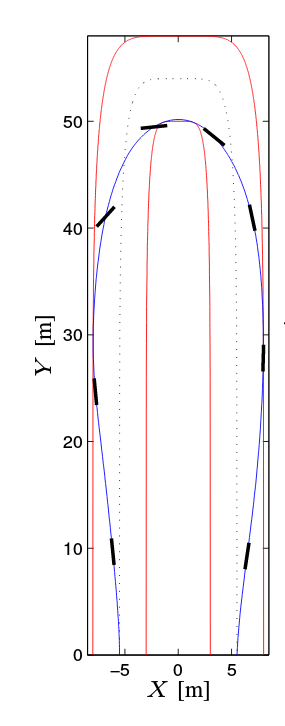
\includegraphics[width=\linewidth, trim=1.5cm 0cm 0cm 0cm]{hairpin.png}
\end{figure}
\end{columns}
\end{frame}

\begin{frame}
\frametitle{Time discretization}
\begin{itemize}
\item
Discretize dynamics with collocation (Radau5)
\item
Can either discretize the full DAE, or the transformed explicit ODE
\item
Interested in how this transformation affects optimization performance
\item
Experience is that the explicit ODE formulation usually is superior
\begin{itemize}
\item
Requires fewer iterations
\item
Cheaper iterations
\item
More likely to succeed
\end{itemize}
\end{itemize}
\end{frame}

\begin{frame}
\frametitle{Implicit vs. explicit}
\begin{itemize}
\item
Want to understand why explicit ODE formulation is superior
\item
Probably not as simple as the problem being smaller
\item
Have noticed that the ODE formulation also is superior for simulation purposes
\item
If you help us understand why, maybe we can understand why ODE formulation is superior for optimization
\end{itemize}
\end{frame}

\begin{frame}
\frametitle{Equations}
{\small
Chassis dynamics (7 equations):
\begin{align}
\dot{v}^X - v^Y \dot{\psi}  &= F_g^x \\
F_g^x &= \frac{1}{m} ( F^x_{f}\cos(\delta) + F^x_{r} -F^y_{f}\sin(\delta) ) \\
\dot{v}^Y + v^X \dot{\psi}  &= F_g^y \\
F_g^y &= \frac{1}{m} ( F^y_{f}\cos(\delta) +
F^y_{r} +F^x_{f}\sin(\delta) ) \\
I_{ZZ} \ddot{\psi} &= M_g^z \\
M_g^z &= l_f F^y_{f}\cos(\delta) - l_r F^y_{r} + l_fF^x_{f}\sin(\delta)
\end{align}

Nominal tire forces (4 equations):
	\begin{align}
		F^x_{0} &= \mu_x F^z 
		\sin\Big( C_{x} 
		\arctan\big(B_{x} \lambda_i -E_{x}(B_{x}\lambda-\arctan B_{x}\lambda)\big)\Big)
		\\ 
		F^y_{0} &= \mu_y F^z \sin\Big( C_{y} \arctan\big(B_{y} \alpha -E_{y}(B_{y}\alpha-\arctan B_{y}\alpha)\big)\Big)
	\end{align}
}
\end{frame}

\begin{frame}
\frametitle{Equations cont.}
{\small

Actual tire forces (12 equations):
\begin{align}
F^{x,y} &= F^{x,y}_{0} G_{m}  \\
G_{m} &= \cos( C_{m} \arctan(H_{m} m) ) \\
H_{m} &= B_{m 1} \cos(\arctan(B_{m 2} m))
\end{align}

Wheel dynamics (2 equations):
\begin{equation}
\tau = I_w \dot{\omega}-R_wF^x,
\end{equation}
}
\end{frame}

\begin{frame}
\frametitle{Equation cont.}
{\small
Slip (4 equations):
	\begin{align}
		\dot{\alpha}_i \frac{\sigma}{v^x_{i}} + \alpha_i &:= -\arctan \left( \frac{v^y_{i}}{v^x_{i}} \right) \label{eq:alpha}\\
		%\lambda_f &= \frac{R_e \omega_f - v_{x,f}}{v_{x,f}}, \label{eq:lambdaf} \\
		%\lambda_r &= \frac{R_e \omega_r - v_{x,r}}{v_{x,r}}, \label{eq:lambdar} \\
		%v_{x,f} &= v_x \cos(\delta) + (v_y + l_f \dot{\psi}) \sin(\delta), \\
		%v_{x,r} &= v_x,\label{eq:vw}
		\lambda_i &:= \frac{R_w \omega_i - v^x_{i}}{v^x_{i}}\label{eq:lambda} 
	\end{align}\label{eq:slip}%

Vehicle sideslip (1 equation):
\begin{gather} %\label{eq:Fz0}
\beta = \arctan\left(\frac{v^Y}{v^X}\right)
\end{gather}

Velocities (3 equations):
\begin{gather}
v_f^x = v^X\cos(\delta) + (v^Y+l_f\dot \psi)\sin(\delta) \\
\dot X = v^X\cos(\psi) - v^Y\sin(\psi) \\
\dot Y = v^X\sin(\psi) + v^Y\cos(\psi)
\end{gather}
}
\end{frame}

\begin{frame}
\frametitle{BLT form}
\begin{figure}[ht]
\centering
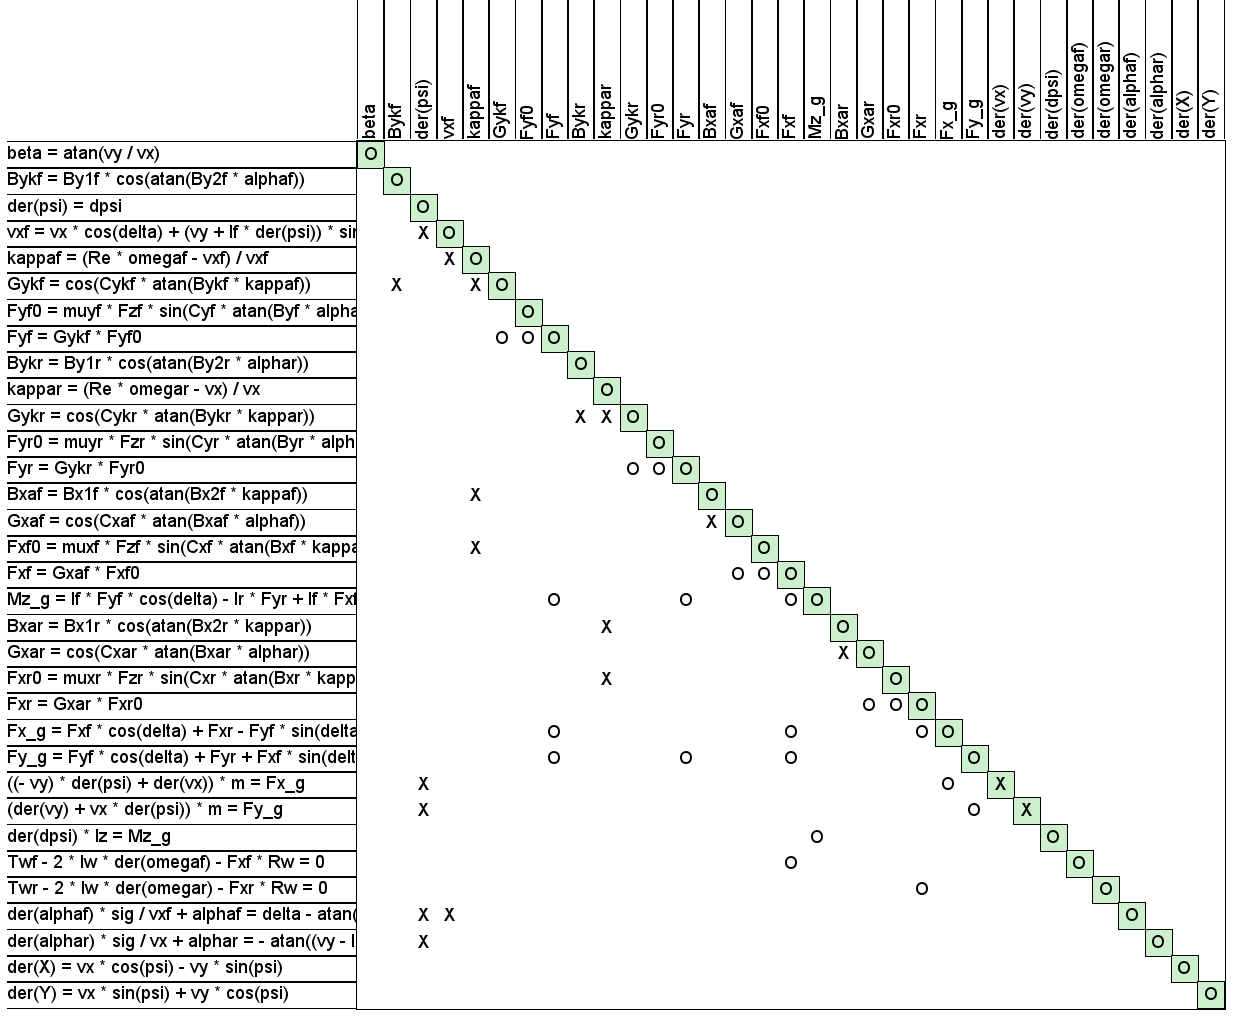
\includegraphics[width=0.84\linewidth]{blt.png}
\end{figure}
\end{frame}

\begin{frame}
\frametitle{Implementation}
\begin{itemize}
\item
We do not utilize JModelica's BLT and FMI framework
\item
Instead transfer the full symbolic DAE to CasADi Interface
\item
Perform our own BLT and ODE transformation using CasADi
\item
Then hook up the causalized system either to JModelica's collocation for optimization or Assimulo for simulation
\item
Can skip our own ODE transformation to expose the full DAE to the optimization or Assimulo
\end{itemize}
\end{frame}

\begin{frame}
\frametitle{Simulation results}
\begin{table}
\centering
\begin{tabular}{lccc}
\toprule
Setup & Time [s] & Steps [1000] & Evals [1000] \\
\midrule
IDA DAE & 43.4 & 33 & 674 \\
IDA DAE sup. alg. & 1.4 & 1.5 & 21 \\
IDA ODE & 0.5 & 1.8 & 8 \\
Radau5 DAE & 5.7 & 2.0 & 51 \\
Radau5 ODE & 0.4 & 0.2 & 4 \\
\bottomrule
\end{tabular}
\end{table}
\end{frame}

\begin{frame}[fragile]
\frametitle{IDA DAE}
{\small
\begin{verbatim}
Final Run Statistics: --- 

 Number of steps                                 : 32885
 Number of function evaluations                  : 67297
 Number of Jacobian evaluations                  : 18383
 Number of function eval. due to Jacobian eval.  : 606639
 Number of error test failures                   : 7482
 Number of nonlinear iterations                  : 67297
 Number of nonlinear convergence failures        : 0

Solver options:

 Solver                       : IDA (BDF)
 Maximal order                : 5
 Suppressed algebr. variables : False
 Tolerances (absolute)        : 1e-06
 Tolerances (relative)        : 1e-08
\end{verbatim}
}
\end{frame}

\begin{frame}[fragile]
\frametitle{IDA DAE sup. alg.}
{\small
\begin{verbatim}
Final Run Statistics: --- 

 Number of steps                                 : 1405
 Number of function evaluations                  : 3897
 Number of Jacobian evaluations                  : 525
 Number of function eval. due to Jacobian eval.  : 17325
 Number of error test failures                   : 215
 Number of nonlinear iterations                  : 3897
 Number of nonlinear convergence failures        : 0

Solver options:

 Solver                       : IDA (BDF)
 Maximal order                : 5
 Suppressed algebr. variables : True
 Tolerances (absolute)        : 1e-06
 Tolerances (relative)        : 1e-08
\end{verbatim}
}
\end{frame}

\begin{frame}[fragile]
\frametitle{IDA ODE}
{\small
\begin{verbatim}
Final Run Statistics: --- 

 Number of steps                                 : 1789
 Number of function evaluations                  : 2972
 Number of Jacobian evaluations                  : 458
 Number of function eval. due to Jacobian eval.  : 4580
 Number of error test failures                   : 271
 Number of nonlinear iterations                  : 2972
 Number of nonlinear convergence failures        : 0

Solver options:

 Solver                       : IDA (BDF)
 Maximal order                : 5
 Suppressed algebr. variables : True
 Tolerances (absolute)        : 1e-06
 Tolerances (relative)        : 1e-08
\end{verbatim}
}
\end{frame}

\begin{frame}[fragile]
\frametitle{Radau5 DAE}
{\small
\begin{verbatim}
Final Run Statistics: --- 

 Number of steps                                 : 1999
 Number of function evaluations                  : 17855
 Number of Jacobian evaluations                  : 1009
 Number of function eval. due to Jacobian eval.  : 33297
 Number of error test failures                   : 585
 Number of LU decompositions                     : 2264

Solver options:

 Solver                  : Radau5 (implicit)
 Tolerances (absolute)   : [  1.00000000e-06]
 Tolerances (relative)   : 1e-08
\end{verbatim}
}
\end{frame}

\begin{frame}[fragile]
\frametitle{Radau5 ODE}
{\small
\begin{verbatim}
Final Run Statistics: --- 

 Number of steps                                 : 207
 Number of function evaluations                  : 1994
 Number of Jacobian evaluations                  : 192
 Number of function eval. due to Jacobian eval.  : 1920
 Number of error test failures                   : 31
 Number of LU decompositions                     : 240

Solver options:

 Solver                  : Radau5 (implicit)
 Tolerances (absolute)   : [  1.00000000e-06]
 Tolerances (relative)   : 1e-08
\end{verbatim}
}
\end{frame}

\begin{frame}[fragile]
\frametitle{Error}
\begin{itemize}
\item
ODE formulation behaves similarly to DAE formulation with suppressed algebraics (faster since Jacobian computation is cheaper)
\item
Does this mean we lose accuracy in the algebraics with the ODE formulation?
\item
First compute ``reference'' solution $\dot x, x, y$ with DAE formulation and \verb|RTOL=1e-12, ATOL=1e-8|
\item
Compare this with DAE, DAE sup. alg., and ODE with default tolerances
\item
Compute relative error as function of time for each variable kind:
\[e_v(t) = \left|\left|\frac{v(t) - \hat v(t)}{v(t) + \epsilon_{\text{mach}}}\right|\right|_\infty, \quad \forall v \in \{\dot x, x, y\}\]
\end{itemize}
\end{frame}

\begin{frame}
\frametitle{Variable kind errors}
\begin{figure}[ht]
\centering
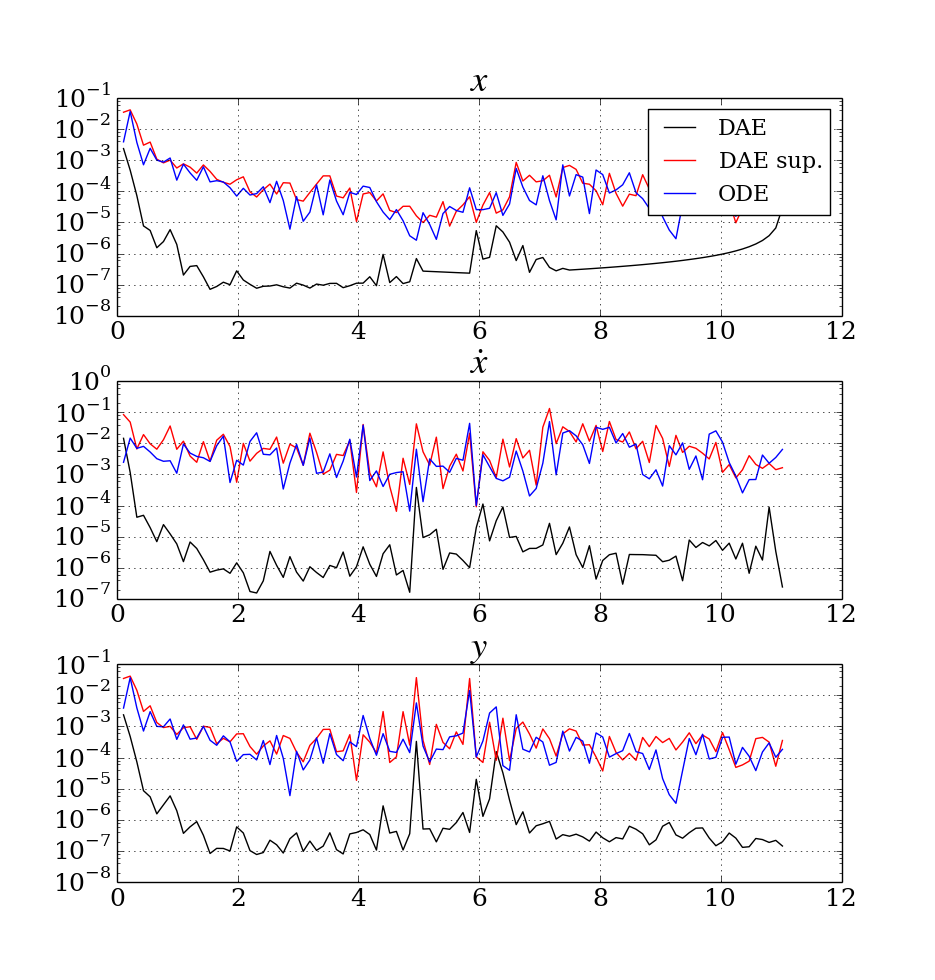
\includegraphics[width=0.73\linewidth]{errors2.png}
\end{figure}
\end{frame}

\begin{frame}
\frametitle{Variable kind errors}
\begin{itemize}
\item
Very roughly speaking, suppressing algebraics or transforming to ODE increases relative error from $10^{-6}$ to $10^{-3}$ for all variable kinds.
\item
Unexpected?
\end{itemize}
\end{frame}

\begin{frame}
\frametitle{Optimization?}
\begin{itemize}
\item
We hoped that understanding these things would help us understand why ODE is good for optimization
\item
But now I think that these are separate issues, since we have fixed step length in optimization
\item
Some tolerance levels start giving nonlinear convergence failures for DAE
\begin{itemize}
\item
Unfortunately, unable to reproduce
\item
Could be related to what we are seeing in optimization?
\item
Is it worth analyzing (if we manage to reproduce)?
\item
Problem conditioning is not straightforward to measure in optimization, but it seems like there is no significant difference between the formulations in this regard
\end{itemize}
\end{itemize}
\end{frame}

\end{document} 
